
\documentclass[twoside,12pt]{article}

\usepackage{dsctemplate}
\usepackage[margin=1in]{geometry}
\usepackage{amsmath}
\usepackage{amssymb,amsthm}
\usepackage{fancyhdr}
\usepackage{nicefrac}
\usepackage{minted}
\usetikzlibrary{quotes,angles,positioning,arrows.meta}
\usetikzlibrary{calc}
\usepackage{enumitem}
\usepackage{fancyvrb}
\usepackage{dirtytalk}
\usepackage{comment}
\usepackage{graphicx}

\DefineVerbatimEnvironment{verbatim}{Verbatim}{xleftmargin=.5in}
\newlist{multiplechoice}{itemize}{2}
\setlist[multiplechoice]{label=$\square$}

\newcommand{\nishant}[1]{{\color{orange}[{\bf Nishant}: #1]}}
\newcommand{\jack}[1]{{\color{purple}[{\bf Jack}: #1]}}
\newcommand{\suraj}[1]{{\color{blue}[{\bf Suraj}: #1]}}


% configuration
% ------------------------------------------------------------------------------

% control whether solutions are shown or hidden
\showsolntrue

% page headers only on odd pages
\pagestyle{fancy}
\fancyhead{}
\fancyhead[RO]{PID: \rule{3in}{.5pt}}
\renewcommand{\headrulewidth}{0pt}
% \pagenumbering{gobble}

% ------------------------------------------------------------------------------

\begin{document}


\thispagestyle{empty}

\vspace{-5.5in}

\pstitle{%
    Final Exam
}{DSC 40A, Summer 2024}

\vspace{-.3in}

\begin{tabular}{rl}
    Full Name: & \inlineresponsebox[4in]{Solutions}\\
    PID: & \inlineresponsebox[4in]{A12345678}\\
    % Seat Number: & \inlineresponsebox[4in]{A1}
    % Lecture: & \bubble{A (10AM)} \bubble{B (9AM)} \bubble{C (1PM)} \bubble{D (8AM)} \vspace{.3in} \\ 
\end{tabular}

\vspace{.1in}

\hline

\vspace{.1in}


\textbf{Instructions:}
    \begin{itemize}
        \item This exam consists of 9 questions, worth a total of 108 points. \textbf{All questions on the exam count towards your Final Exam score, but Questions 1-4 count towards your Midterm Redemption score.} \textit{Advice: Read all of the questions before starting to work, because the questions are not sorted by difficulty.}
        \item Write your PID in the top right corner of each page in the space provided.
        \item Please write \textbf{clearly} in the provided answer boxes; we will not grade work that appears elsewhere.
        \begin{itemize}
            \item For questions that ask you to show your work, correct answers with no work shown will receive no credit.
            \item When asked to do so, please place your final answer in a $\boxed{\text{box}}$.
            \item \bubble{In multiple choice questions, select only one option and completely fill in the corresponding bubble --- if we cannot tell which option you selected, you may not receive credit.}
            \item \squarebubble{A square box means you should \textbf{select all that apply}. Completely fill in all boxes that apply.}

        \end{itemize}
        \item You may refer to two two-sided index cards of maximum size 4 inches by 6 inches that you wrote on by hand and by yourself. Other than that, you may not refer to any resources or technology during the exam (no phones, no smart watches, no computers, and no calculators).
    \end{itemize}

\vspace{.1in}

\hline

\vspace{.2in}

\noindent By signing below, you are agreeing that you will behave honestly and fairly during
and after this exam. 

\begin{tabular}{rl}
    \: \: \: \: \: Signature: & \inlineresponsebox[4in]{}\\
\end{tabular}

\vfill

\begin{center}
{\huge Version B} \vspace{.2in}

Please do not open your exam until instructed to do so.

\end{center}

\newpage

\begin{probset}

\begin{prob}[(19 pts) \small{\textbf{[Eligible for midterm redemption]}}]
Consider the dataset $x_1 = 1, x_2 = 2, x_3 = 3, x_4 = 4, x_5 = 5$.

% \nishant{remove labels from losses?} \suraj{good idea}

\begin{subprobset}
    \begin{subprob} (3 pts)
        Which single element of the dataset would you change, and to what value, to make \( h^* = 4 \) the single minimizing value for the following loss function and corresponding empirical risk? Bubble in your choice of $x_i$, if possible, and provide the new value of that $x_i$ in the box below. If no such $x_i$ is possible, bubble in ``Not possible" and explain why in the box below.
        % $$L_{0,1}(y_i, h) = \begin{cases} 0 & y_i = h \\ 1 & y_i \neq h \end{cases}$$
        $$L(y_i, h) = \begin{cases} 0 & y_i = h \\ 1 & y_i \neq h \end{cases}$$

        \begin{center}
            \bubble{$x_1$}
            \bubble{$x_2$}
            \bubble{$x_3$}
            \correctbubble{$x_4$}
            \bubble{$x_5$}
            \bubble{Not possible}
        \end{center}
        \begin{responsebox}{0.65in}
            
        \end{responsebox}
    \end{subprob}
    
    \begin{subprob}(2 pts)
        Suppose we must modify $x_5$. What should the new value of $x_5$ be to make \( h^* = 6 \) for the following loss function and corresponding empirical risk?  
        % \suraj{I feel like it's more accurate to say ``for the following empirical risk function". This is also inconsistent with the previous question, where you just showed the loss --- either show the loss in all or the ER in all for consistency.}

        % $$R_\text{sq}(h) = \frac{1}{n} \sum_{i = 1}^n (y_i - h)^2$$
        \vspace{-0.3cm}
        $$L(y_i, h) = (y_i - h)^2$$

        \begin{center}
            $x_5 = $\inlineresponsebox[3in]{}
        \end{center}
    \end{subprob}
    
    \begin{subprob}(2 pts)
        Suppose we must modify $x_1$. What should the new value of $x_1$ be to make \( h^* = 6 \) for the following loss function and corresponding empirical risk? 

        % $$R_\text{sq}(h) = \frac{1}{n} \sum_{i = 1}^n (y_i - h)^2$$
        \vspace{-0.3cm}
        $$L(y_i, h) = (y_i - h)^2$$
        \begin{center}
            $x_1 = $\inlineresponsebox[3in]{}
        \end{center}
    \end{subprob}

\end{subprobset}

\newpage 
\textit{The following information is repeated from the previous page, for your convenience.} 

Consider the dataset $x_1 = 1, x_2 = 2, x_3 = 3, x_4 = 4, x_5 = 5$.

\begin{subprobset}

    \begin{subprob}(3 pts)
        Which single element of the dataset would you change, and to what value, to make \( h^* = 4 \) for the following loss function and corresponding empirical risk? Bubble in your choice of $x_i$, if possible, and provide the new value of that $x_i$ in the box below. If no such $x_i$ is possible, bubble in ``Not possible" and explain why in the box below.
% $$R_\text{abs}(h) = \frac{1}{n} \sum_{i = 1}^n |y_i - h|$$
$$L(y_i, h) = |y_i - h|$$
        \begin{center}
            \bubble{$x_1$}
            \bubble{$x_2$}
            \bubble{$x_3$}
            \bubble{$x_4$}
            \bubble{$x_5$}
            \bubble{Not possible}
        \end{center}
        \begin{responsebox}{0.75in}
            
        \end{responsebox}
    \end{subprob}
    
    \begin{subprob}(3 pts)
        Which single element of the dataset would you change, and to what value, to make \( h^* = 5 \) for the following loss function and corresponding empirical risk? Bubble in your choice of $x_i$, if possible, and provide the new value of that $x_i$ in the box below. If no such $x_i$ is possible, bubble in ``Not possible" and explain why in the box below.
% $$R_\text{abs}(h) = \frac{1}{n} \sum_{i = 1}^n |y_i - h|$$
$$L(y_i, h) = |y_i - h|$$

        \begin{center}
            \bubble{$x_1$}
            \bubble{$x_2$}
            \bubble{$x_3$}
            \bubble{$x_4$}
            \bubble{$x_5$}
            \bubble{Not possible}
        \end{center}
        \begin{responsebox}{0.75in}
            
        \end{responsebox}
    \end{subprob}

    \begin{subprob}(2 pts)
        Suppose we \textbf{delete} $x_2$, so the dataset is $x_1 = 1, x_3=3, x_4=4, x_5=5$. What is the new value of $h^*$ for following loss function and corresponding empirical risk?
        % $$R_\text{sq}(h) = \frac{1}{n} \sum_{i = 1}^n (y_i - h)^2$$
        $$L(y_i, h) = (y_i - h)^2$$

        \begin{center}
            $h^* = $ \inlineresponsebox[3in]{}
        \end{center}
    \end{subprob}

    
    \begin{subprob}(4 pts)
        Suppose we \textbf{delete} $x_3$, so the dataset is $x_1 = 1, x_2=2, x_4=4, x_5=5$. Which of the following values of $h^*$ minimize the following loss function and corresponding empirical risk? 
        % $$R_\text{abs}(h) = \frac{1}{n} \sum_{i = 1}^n |y_i - h|$$
        $$L(y_i, h) = |y_i - h|$$
        
        % \begin{center}
        %     \squarebubble{1} \hspace{-0.7cm}
        %     \squarebubble{1.5} \hspace{-0.7cm}
        %     \correctsquarebubble{2} \hspace{-0.7cm}
        %     \correctsquarebubble{2.5} \hspace{-0.7cm}
        %     \correctsquarebubble{3} \hspace{-0.7cm}
        %     \correctsquarebubble{3.5} \hspace{-0.7cm}
        %     \correctsquarebubble{4} \hspace{-0.7cm}
        %     \squarebubble{4.5} \hspace{-0.7cm}
        %     \squarebubble{5} \hspace{-0.7cm}
        % \end{center}
    \end{subprob}
\end{subprobset}
\end{prob}

% \suraj{I didn't work this out fully so take it with a grain of salt --- I believe that you'd answer parts (f) and (g), or some variants of them, on the way to answering parts (b), (c), ..., meaning that the earlier parts are easier than the later parts. I might reverse that?}

\newpage

\begin{prob}[(12 pts) \small{\textbf{[Eligible for midterm redemption]}}]

% \suraj{Isn't this ripped straight from the Spring 2024 Final lmao. I'd perhaps center the ER functions with double dollar signs.}
% \nishant{Jack said same setup with the datasets but different questions}
    
    Consider a dataset of 4 values, $y_1 < y_2 < y_3 < y_4$, with a mean of 6. \\ Let $Y_\text{abs}(h) = \frac{1}{4} \sum_{i = 1}^4 |y_i - h|$ represent the mean absolute error of a constant prediction $h$ on this dataset of 4 values.

    Similarly, consider another dataset of 3 values, $x_1 < x_2 < x_3$, that also has a mean of 6. \\ Let $X_\text{abs}(h) = \frac{1}{3} \sum_{i = 1}^3 |x_i - h|$ represent the mean absolute error of a constant prediction $h$ on this dataset of 3 values.

    Suppose that $x_1 < y_1$, $y_4 < x_2$, and that $T_\text{abs}(h)$ represents the mean \textbf{absolute} error of a constant prediction $h$ on the combined dataset of 7 values, $x_1, y_1, ..., y_4, x_2, x_3$. We denote these 7 values as $\{ z_1, z_2, z_3, z_4, z_5, z_6, z_7 \}$.


    \begin{subprobset}
        \begin{subprob}(2 pts)
            What value of $h$ minimizes the following empirical risk function? $$Z(h) = \frac{1}{7} \sum_{i = 1}^7 (h - z_i)$$

            % \suraj{Mean error is not a term they know of. Clever idea, though. Don't use the same letter $T$ for this, since you defined that to mean MAE. This is tricky in part because since there's no absolute value/square, it matters whether it's $h - z_i$ or $z_i - h$. Also, the $z$s are never defined anywhere.}
            
            \correctbubble{$-\infty$}
            
            \bubble{0}
            
            \bubble{6}
            
            \bubble{$y_3$}
            
            \bubble{Any value between $y_3$ and $y_4$}
            
            % \bubble{$\infty$}
            
        \end{subprob}

        \begin{subprob}(2 pts)
            What value of $h$ minimizes \textbf{mean absolute error}, $T_\text{abs}(h)$?
            
            \bubble{$-\infty$}
            
            \bubble{0}

            \bubble{6}
            
            \correctbubble{$y_3$}
            
            \bubble{Any value between $y_3$ and $y_4$}
            
            \bubble{$\infty$}
            
        \end{subprob}

        \vspace{1em}


\end{subprobset}        

        % \suraj{The language is a little casual here.}
        
        Suppose the slope of $T_\text{abs}(h)$ is $-\frac{1}{7}$ at some $h_p$. \textit{Hint: think about what values of $h$ could have this slope.}
\begin{subprobset}
        \begin{subprob}(3 pts)
        Suppose the dataset is now modified by moving the $\{x_i\}$ such that \\  $y_1 < y_2 < y_3 < y_4 < x_1 < x_2 < x_3$. 
        What would the slope of $T_\text{abs}(h)$ be \textbf{at the point whose $x$-value is $h_p$}, given this assumption?

        \begin{responsebox}{0.5in}
            -\frac{3}{7}
        \end{responsebox}
            \end{subprob}


\end{subprobset}
\newpage
    \textit{The following information is repeated from the previous page, for your convenience.} 
    
    Consider a dataset of 4 values, $y_1 < y_2 < y_3 < y_4$, with a mean of 6. Let $Y_\text{abs}(h) = \frac{1}{4} \sum_{i = 1}^4 |y_i - h|$ represent the mean absolute error of a constant prediction $h$ on this dataset of 4 values.

    Similarly, consider another dataset of 3 values, $x_1 < x_2 < x_3$, that also has a mean of 6. Let $X_\text{abs}(h) = \frac{1}{3} \sum_{i = 1}^3 |x_i - h|$ represent the mean absolute error of a constant prediction $h$ on this dataset of 3 values.

    Suppose that $x_1 < y_1$, $y_4 < x_2$, and that $T_\text{abs}(h)$ represents the mean \textbf{absolute} error of a constant prediction $h$ on the combined dataset of 7 values, $x_1, y_1, ..., y_4, x_2, x_3$. We denote these 7 values as $\{ z_1, z_2, z_3, z_4, z_5, z_6, z_7 \}$.

    Suppose the slope of $T_\text{abs}(h)$ is $-\frac{1}{7}$ at some $h_p$. \textit{Hint: think about what values of $h$ could have this slope.}

\begin{subprobset}
    
        \begin{subprob}(3 pts)
            Suppose the dataset is now modified by repeating each value $y_i$ such that it now contains $x_1, y_1, y_1, y_2, y_2, y_3, y_3, y_4, y_4$, in ascending order; the ordering of the points is the same as the beginning of this question. What would the slope of $T_\text{abs}(h)$ be \textbf{at the point whose $x$-value is $h_p$}, given this assumption?

            \begin{responsebox}{0.5in}
            
        \end{responsebox}
        
        \end{subprob}

        \begin{subprob}(3 pts)
            \textbf{At the point whose $x$-value is $h_{p}$}, select the option below that correctly describes the relationship between the \textbf{slopes} of $Y_\text{abs}(h)$, $X_\text{abs}(h)$, and $T_\text{abs}(h)$, respectively.

            \textit{Hint: We already know the slope of $T_\text{abs}(h)$ at $h_p$.}

            \vspace{0.2em}

            \bubble{$\text{slope of }Y_\text{abs}(h) < \text{slope of } T_\text{abs}(h) < \text{slope of } X_\text{abs}(h)$}

            \bubble{$\text{slope of }Y_\text{abs}(h) < \text{slope of } X_\text{abs}(h) < \text{slope of } T_\text{abs}(h)$}

            \bubble{$\text{slope of }T_\text{abs}(h) < \text{slope of } X_\text{abs}(h) < \text{slope of } Y_\text{abs}(h)$}

            \bubble{$\text{slope of }T_\text{abs}(h) < \text{slope of } Y_\text{abs}(h) < \text{slope of } X_\text{abs}(h)$}

            \correctbubble{$\text{slope of }X_\text{abs}(h) < \text{slope of } T_\text{abs}(h) < \text{slope of } Y_\text{abs}(h)$}

            \bubble{$\text{slope of }X_\text{abs}(h) < \text{slope of } Y_\text{abs}(h) < \text{slope of } T_\text{abs}(h)$}

            
        \end{subprob}
        
    \end{subprobset}
    
\end{prob}


\newpage \begin{prob}[(17 pts) \small{\textbf{[Eligible for midterm redemption]}}]

Consider the following vectors in \( \mathbb{R}^3 \), where $\alpha \in \mathbb{R}$ is a scalar:

\[
\vec{v}_1 = \begin{bmatrix} 0 \\ 1 \\ 1 \end{bmatrix}, \quad 
\vec{v}_2 = \begin{bmatrix} 1 \\ 0 \\ 1 \end{bmatrix}, \quad 
\vec{v}_3 = \begin{bmatrix} \alpha \\ 1 \\ 2 \end{bmatrix}
\]

\begin{subprobset}        
    \begin{subprob}(2 pts)
        For what value(s) of $\alpha$ are $\vec{v}_1, \vec{v}_2,$ and $\vec{v}_3$ linearly independent? Show your work, and put your answer in a \boxed{\text{box}}. 

\begin{responsebox}{1.32in}

\end{responsebox}
    \end{subprob}
    
    \begin{subprob}(2 pts)
        For what value(s) of $\alpha$ are $\vec{v}_1$ and $\vec{v}_3$ orthogonal? Show your work, and put your answer in a \boxed{\text{box}}. 

\begin{responsebox}{1.32in}

\end{responsebox}
    \end{subprob}
    
    \begin{subprob}(2 pts)
        For what value(s) of $\alpha$ are $\vec{v}_2$ and $\vec{v}_3$ orthogonal? Show your work, and put your answer in a \boxed{\text{box}}. 

\begin{responsebox}{1.32in}

\end{responsebox}
    \end{subprob}

    \begin{subprob}(2 pts)
        Regardless of your answer above, assume in this part that $\alpha = 3$. Is the vector $\begin{bmatrix}
3 \\
5 \\
8
\end{bmatrix}$ in $\textbf{span}(\vec{v}_1, \vec{v}_2, \vec{v}_3)$?
\vspace{-0.3cm}
    \begin{center}
        \correctbubble{Yes} 
        \bubble{No}
    \end{center}
    \end{subprob}
\end{subprobset}
\newpage 
\textit{The following information is repeated from the previous page, for your convenience.} 

Consider the following vectors in \( \mathbb{R}^3 \), where $\alpha \in \mathbb{R}$ is some scalar:

\[
\vec{v}_1 = \begin{bmatrix} 0 \\ 1 \\ 1 \end{bmatrix}, \quad 
\vec{v}_2 = \begin{bmatrix} 1 \\ 0 \\ 1 \end{bmatrix}, \quad 
\vec{v}_3 = \begin{bmatrix} \alpha \\ 1 \\ 2 \end{bmatrix}
            \]
\begin{subprobset}

    \vspace{0.3cm}
    \begin{subprob}(2 pts)
        What is the projection of the vector $\begin{bmatrix}
3 \\
5 \\
8
\end{bmatrix}$ onto $\vec{v}_1$? Provide your answer in the form of a vector. Show your work, and put your answer in a \boxed{\text{box}}. 
    % \suraj{Specify what form they should give their answer as --- is this the scalar weighting or the new vector itself. Depending on the class, this means different things. Needs an answer box of some sort too.}

    \begin{responsebox}{3in}
        
    \end{responsebox}
    \end{subprob} 

\end{subprobset}
\newpage
\textit{The following information is repeated from the previous page, for your convenience.} 

Consider the following vectors in \( \mathbb{R}^3 \), where $\alpha \in \mathbb{R}$ is some scalar:

\[
\vec{v}_1 = \begin{bmatrix} 0 \\ 1 \\ 1 \end{bmatrix}, \quad 
\vec{v}_2 = \begin{bmatrix} 1 \\ 0 \\ 1 \end{bmatrix}, \quad 
\vec{v}_3 = \begin{bmatrix} \alpha \\ 1 \\ 2 \end{bmatrix}
            \]
\begin{subprobset}
\begin{subprob}(4 pts)
        What is the orthogonal projection of the vector $\begin{bmatrix}
3 \\
15 \\
18
\end{bmatrix}$ onto $\textbf{span}(\vec{v}_1, \vec{v}_2)$? Note that for $X = \begin{bmatrix}
            0 & 1 \\ 1 & 0 \\ 1 & 1
        \end{bmatrix}$, we have 

        $$(X^T X) ^{-1}X^T = \begin{bmatrix}
            -\frac{1}{3} & \frac{2}{3} & \frac{1}{3} \\[6pt]
            \frac{2}{3} & -\frac{1}{3} & \frac{1}{3}  
        \end{bmatrix}$$ 
        Write your answer in the form of coefficients that multiply $\vec{v}_1$ and $\vec{v}_2$ and yield a vector $\vec{p}$ that is the orthogonal projection requested above.
        \begin{center}
            $\vec{p} = \inlineresponsebox[1.5in]{}\cdot \vec{v}_1 + \inlineresponsebox[1.5in]{}\cdot \vec{v}_2$
        \end{center}
    \end{subprob}
\bigskip
    \begin{subprob}(3 pts)
        Is it true that, for the orthogonal projection $\vec{p}$ from above, the entries of \\ $\vec{e} = \vec{p} \ - \begin{bmatrix} 3 \\ 15 \\ 18 \end{bmatrix}$ sum to $0$? Explain why or why not. Your answer must mention characteristics of $\vec{v}_1,\vec{v}_2,$ and/or $X$ to receive full credit.

        \begin{center}
            \bubble{Yes}
            \correctbubble{No}
        \end{center}

        \begin{responsebox}{1.2in}
            
        \end{responsebox}
    \end{subprob}

\end{subprobset}

\end{prob}

\newpage \begin{prob}[(13 pts) \small{\textbf{[Eligible for midterm redemption]}}]

You are given a dataset with the following data points and want to fit a variety of hypothesis functions to predict $y$ from features $u$ and $v$:

\[
\begin{array}{|c|c|c|}
\hline
u & v & y \\
\hline
1 & 3  & 4  \\
3 & 0  & 6  \\
2 & 2  & 5  \\
4 & -4 & 8  \\
5 & -1 & 11 \\
\hline
\end{array}
\]

% \suraj{Also, make it so that a question and its answer choices are always on the same page, perhaps repeating necessary info on the next page.}

You are also provided with the following hypothesis functions, used to construct design matrices: 
% \nishant{double-check design matrices}

% \nishant{Should these be lists of features, not hypothesis functions, and then we can shuffle the design matrices to make it harder?}


\begin{enumerate}
    \item $H_A(u, v) = w_0 + w_1 u + w_2 u^2 + w_3 u^3$
    
    
    \item $H_B(u, v) = w_0 u + w_1 u^2 + w_2 u^3 + w_3 u v$

    \item $H_C(u, v) = w_0 + w_1 u + w_2 v + w_3 v^2$
    
    \item $H_D(u, v) = w_0 + w_1 u + w_2 u^3 + w_3 u v$
\end{enumerate}
% $$
%     X_1 = \begin{bmatrix}
%     1 &  1 & 1 & 1 \\
%     1 &  3 & 9 & 27 \\
%     1 &  2 & 4 & 8 \\
%     1 &  4 & 16 & 64 \\
%     1 &  5 & 25 & 125
%     \end{bmatrix} \ \ \ 
%     X_2 = \begin{bmatrix}
%     1 & 1 & 1 & 3 \\
%     1 & 9 & 27 & 0 \\
%     1 & 4 & 8 & 4 \\
%     1 & 16 & 64 & -16 \\
%     1 & 25 & 125 & -5
%     \end{bmatrix} 
% $$ 
% $$
%     X_3 = \begin{bmatrix}
%     1 & 1 & 3  & 9 \\
%     1 & 3 & 0  & 0 \\
%     1 & 2 & 2  & 4 \\
%     1 & 4 & -4 & 16 \\
%     1 & 5 & -1 & 1
%     \end{bmatrix} \ \ \ 
%     X_4 = \begin{bmatrix}
%     1 & 1 & 1   & 3 \\
%     1 & 3 & 27  & 0 \\
%     1 & 2 & 8   & 4 \\
%     1 & 4 & 64  & -16 \\
%     1 & 5 & 125 & -5
%     \end{bmatrix}
% $$
$$
    X_1 = \begin{bmatrix}
    1 &  1 & 1 & 1 \\
    1 &  3 & 9 & 27 \\
    1 &  2 & 4 & 8 \\
    1 &  4 & 16 & 64 \\
    1 &  5 & 25 & 125
    \end{bmatrix} \ \ \ 
    X_2 = \begin{bmatrix}
    1 & 1 & 1   & 3 \\
    1 & 3 & 27  & 0 \\
    1 & 2 & 8   & 4 \\
    1 & 4 & 64  & -16 \\
    1 & 5 & 125 & -5
    \end{bmatrix} 
$$ 
$$
    X_3 = \begin{bmatrix}
    1 & 1 & 1 & 3 \\
    3 & 9 & 27 & 0 \\
    2 & 4 & 8 & 4 \\
    4 & 16 & 64 & -16 \\
    5 & 25 & 125 & -5
    \end{bmatrix} \ \ \ 
    X_4 = \begin{bmatrix}
    1 & 1 & 3  & 9 \\
    1 & 3 & 0  & 0 \\
    1 & 2 & 2  & 4 \\
    1 & 4 & -4 & 16 \\
    1 & 5 & -1 & 1
    \end{bmatrix}
$$
    

\begin{subprobset}
    \begin{subprob}(2 pts)
        Which design matrix corresponds to $H_A(u, v)$?

        \begin{center}
            \correctbubble{$X_1$}
            \bubble{$X_2$}
            \bubble{$X_3$}
            \bubble{$X_4$}
        \end{center}
    \end{subprob}

    \begin{subprob}(2 pts)
        Which design matrix corresponds to $H_B(u, v)$?

        \begin{center}
            \bubble{$X_1$}
            \bubble{$X_2$}
            \correctbubble{$X_3$}
            \bubble{$X_4$}
        \end{center}
    \end{subprob}

    \begin{subprob}(2 pts)
        Which design matrix corresponds to $H_C(u, v)$?

        \begin{center}
            \bubble{$X_1$}
            \bubble{$X_2$}
            \bubble{$X_3$}
            \correctbubble{$X_4$}
        \end{center}
    \end{subprob}

    \begin{subprob}(2 pts)
        Which design matrix corresponds to $H_D(u, v)$?

        \begin{center}
            \bubble{$X_1$}
            \correctbubble{$X_2$}
            \bubble{$X_3$}
            \bubble{$X_4$}
        \end{center}
    \end{subprob}
\end{subprobset}
The following hypothesis functions are repeated from the previous page, for your convenience, plus an additional hypothesis function $H_E$:
\begin{enumerate}
    \item $H_A(u, v) = w_0 + w_1 u + w_2 u^2 + w_3 u^3$
    
    
    \item $H_B(u, v) = w_0 u + w_1 u^2 + w_2 u^3 + w_3 u v$

    \item $H_C(u, v) = w_0 + w_1 u + w_2 v + w_3 v^2$
    
    \item $H_D(u, v) = w_0 + w_1 u + w_2 u^3 + w_3 u v$
    
    \item $H_E(u, v) = w_0 + w_1 u + w_2 u^2 + w_3 u^3 + w_4 v + w_5 v^2 + w_6 u v$
\end{enumerate}
\begin{subprobset}
    \begin{subprob}(3 pts)
        Which of the five hypothesis functions above has the lowest mean squared error on this dataset? Choose a hypothesis function $H(\cdot)$ and briefly justify your answer in the space below.

        \begin{center}
            \bubble{$H_A(u, v)$}
            \bubble{$H_B(u, v)$}
            \bubble{$H_C(u, v)$}
            \bubble{$H_D(u, v)$}
            \bubble{$H_E(u, v)$}
        \end{center}

        \begin{responsebox}{1in}
            
        \end{responsebox}
    \end{subprob}

    \begin{subprob}(2 pts)
        Suppose we use the lowest-MSE hypothesis function chosen above to make a prediction for a new point $(u_\text{new}, v_\text{new}) = (10, 15)$. Is this prediction likely to be accurate? Justify your answer.

        \begin{responsebox}{1in}
            
        \end{responsebox}
    \end{subprob}

\end{subprobset}

% Consider the four design matrices below:


% \vspace{2em}

% $
% A =
% \begin{array}{l}
% \begin{bmatrix}
% -4 & 2 & 1 \\
% 9.5 & 2 & -5 \\
% 0 & 2 & -0.5 \\
% \end{bmatrix}
% \end{array}
% $

% \vspace{1em}

% $
% B =
% \begin{bmatrix}
% -3 & 5 & 7 \\
% 4 & 5.5 & 1 \\
% 2.5 & 2 & -1 \\
% \end{bmatrix}
% $

% \vspace{1em}

% $
% C =
% \begin{bmatrix}
% 2 & -1 & 4 \\
% 6 & 8 & 1 \\
% 1 & -1.5 & 3 \\
% \end{bmatrix}
% $

% \vspace{1em}

% $
% D =
% \begin{bmatrix}
% 1 & 8 & -7 \\
% 1 & 9 & 4.5 \\
% 1 & -3 & 2 \\
% \end{bmatrix}
% $

% \vspace{1em}

% $
% E =
% \begin{bmatrix}
% 2 & 0 & 1 \\
% -1 & 3 & 5 \\
% 3 & -1 & 2 \\
% \end{bmatrix}
% $

% \vspace{1em}

% Select the design matrices where the sum of the entries in the residual (or error) vector (defined as $\vec{e} = \vec{y} - X\vec{w}$) from a linear regression model is guaranteed to be zero. Select all that apply.

% \suraj{I know I suggested this problem, but it seems a bit too complicated. Maybe instead structure it using the relationships in the matrix that Nishant mentioned in his comments. e.g., ``what if the design matrix was such that $x^{(1)} + x^{(2)} = [15, 15, 15]$.}
% ok
% \vspace{0.2em}


% \correctsquarebubble{\text{Matrix A}}

% \nishant{Checking all these for quality to assure correctness. Matrix A has a column of all 2s, which means the residuals will sum to 0.}

% \squarebubble{\text{Matrix B}}

% \nishant{Matrix B is just a full-rank 3x3 Matrix. No linear combination of the columns gives a column of identical numbers, so the sum of the residuals from a linear regression model is not guaranteed to be zero.}

% \squarebubble{\text{Matrix C}}

% \nishant{Matrix C is a matrix where 1.5a - c = the second column (Double-check this for me). However, this is unrelated to whether the residuals will sum to 0, and so the sum of the residuals from a linear regression model is not guaranteed to be zero.}

% \correctsquarebubble{\text{Matrix D}}

% \nishant{Matrix D is a matrix with an intercept term, so the sum of the residuals from a linear regression model is guaranteed to be zero.}

% \correctsquarebubble{\text{Matrix E}}

% \nishant{Matrix E is a matrix where a + c = 2, 2, 2. So, the sum of the residuals from a linear regression model is  guaranteed to be zero.}





\end{prob}

\newpage \begin{prob}[(10 pts)]

Let $\vec{x} = \begin{bmatrix} x_1 \\ x_2 \end{bmatrix}$. Consider the function $g(\vec{x}) = x_1^2 + x_2^2 + x_1 x_2 - 4x_1 - 6x_2 + 8$.
\begin{subprobset}

\begin{subprob}(4 pts) Find $\nabla g(\vec{x})$, the gradient of $g(\vec{x})$, and use it to show that $\nabla g\left( \begin{bmatrix} 1 \\ 2 \end{bmatrix} \right) = \begin{bmatrix} 0 \\ -1 \end{bmatrix}$.

\begin{responsebox}{2.5in}
    
\end{responsebox}

\end{subprob}

\begin{subprob}(4 pts) We'd like to find the vector $\vec{x}^*$ that minimizes $g(\vec{x})$ using gradient descent. Perform one iteration of gradient descent by hand, using the initial guess $\vec{x}^{(0)} = \begin{bmatrix} 1 \\ 2 \end{bmatrix}$ and the learning rate $\alpha = \frac{1}{4}$. Show your work, and put a  $\boxed{\text{box}}$ around your final answer for $\vec{x}^{(1)}$.

\begin{responsebox}{2in}
    
\end{responsebox}
    
\end{subprob}

\newpage \begin{subprob}(3 pts)
    Given some new function $f(x)$ that is convex, prove that the function $g(x) = a f(x) + b$ is also convex, where $a$ and $b$ are positive real constants. 
    
    Note: this function $g(\cdot)$ is entirely different from $g(\vec{x})$ on the previous page.

    % \suraj{Personally not a fan of this sort of question, really just symbol pushing. But given that the exam is Friday, fine to keep}

    \textit{Hint: Use the fact that we already know $f(x)$ is convex and the formal definition of convexity: for all $t\in[0, 1], \ (1-t) f(c) + t f(d) \geq f\left((1-t)c + td\right)$.}

    \begin{responsebox}{2.5in}
            
        \end{responsebox}
\end{subprob}
\end{subprobset}
    
\end{prob}

\newpage

\begin{prob}[(12 pts)]
Euchre is a card game popular in the Midwest United States and is played with a partial deck of 24 cards: the 9, 10, Jack, Queen, King, and Ace of all four suits (Hearts, Diamonds, Spades, Clubs). A hand of cards in Euchre is 5 cards.

Assume cards are dealt by drawing at random \textbf{without replacement} from the set of 24 possible cards. The order of cards in a hand does not matter.

In this question, you may leave your answers unsimplified, in terms of fractions, exponents, factorials, the permutation formula $P(n, k)$, and the binomial coefficient ${n \choose k}$.


\begin{subprobset}
    \begin{subprob}(2 pts)
        How many possible hands of 5 cards are there in total?

        \begin{responsebox}{0.9in}
            
        \end{responsebox}
    \end{subprob}

    
    \begin{subprob}(3 pts)
        What is the probability that all five cards in a hand of Euchre are from the same suit?

        \begin{responsebox}{0.9in}
            
        \end{responsebox}
    \end{subprob}
    
    \begin{subprob}(4 pts)
        What is the probability that exactly two cards in a hand of Euchre are from the same suit?

        \begin{responsebox}{0.9in}
            
        \end{responsebox}
    \end{subprob}

    
    \begin{subprob}(3 pts)
        Euchre is played by four players, so when all cards are dealt, there are four remaining cards ($24 - 4\cdot 5)$. What is the probability that all four remaining cards are Jacks (the strongest card in Euchre)?

        \begin{responsebox}{0.9in}
            
        \end{responsebox}
    \end{subprob}

    
\end{subprobset}
\end{prob}

\newpage \begin{prob}[(11 pts)]
    You go to the (world-renowned) San Diego Safari Park. The animals you see there appear at random, depending on the exhibit. The probabilities of seeing an animal in a given exhibit (Plains, Forest, and Jungle) are provided in the table below. For example, the probability of seeing a Camel if you are in the African Plains is $\frac{3}{5} = 60\%$, and the probability you do not see a Camel if you are in the African Plains is the complement, $\frac{2}{5} = 40\%$. Note that you may see multiple animals in each exhibit, so the probabilities given in each row sum to well over 100\%.

    On the day you go to the Safari Park, the tram navigation system malfunctions and takes you to exhibits at random. It takes guests to the African Plains with probability $\frac{3}{5}$, the Gorilla Forest with probability $\frac{1}{10}$, and the Hidden Jungle with probability $\frac{3}{10}$. 

\begin{table}[h!]
    \centering
    \renewcommand{\arraystretch}{1.6}
    \begin{tabular}{|c|c|c|c|c|c|c|}
        \hline
        \textbf{Location} & \textbf{Rhino} & \textbf{Camel} & \textbf{Gazelle} & \textbf{Lemur}  & \textbf{Fruit Bat}  & \textbf{Gorilla} \\ \hline
        African Plains  & \(\frac{3}{10}\) & \(\frac{3}{5}\) & \(\frac{1}{2}\) & \(\frac{1}{10}\) &  -       & \(\frac{1}{4}\)    \\ \hline
        Gorilla Forest & \(\frac{3}{10}\) & \(\frac{1}{10}\)    & \(\frac{1}{5}\)  & \(\frac{1}{4}\) & \(\frac{7}{20}\)  & \(\frac{9}{20}\) \\ \hline
        Hidden Jungle  & -    & -    & -    & \(\frac{1}{5}\) &  \(\frac{2}{5}\)   & -    \\ \hline
    \end{tabular}    % \caption{Probabilities of Seeing Animals in Different Habitats}
    \label{tab:animal_probs_transposed}
\end{table}

In this question, you may leave your answers unsimplified, in terms of fractions, exponents, factorials, the permutation formula $P(n, k)$, and the binomial coefficient ${n \choose k}$.

% \suraj{There's a lot to read here, and a lot of it feels a little confusing on first read --- I get the premise, but it can be cleaned up a bit. For instance, ``the probabilities sum to well over 100\%" -- which do, the rows or columns? ``but" the animals appear at random, but doesn't seem like the right word. Where you say 60\% I might say $\frac{3}{5} = 60\%$. Overall good question, just needs cleaning up.}

\begin{subprobset}
    \begin{subprob}(2 pts)
        Assume you only go to one exhibit. What is the probability you see a Lemur at the Safari Park? Show your work, and put a \boxed{\text{box}} around your final answer.

        \begin{responsebox}{1in}
            
        \end{responsebox}
    \end{subprob}

    \begin{subprob}(3 pts)
        Assume you only go to one exhibit, and you see a Lemur. What is the probability you are at the African Plains? Show your work, and put a \boxed{\text{box}} around your final answer.

        \begin{responsebox}{1in}
            
        \end{responsebox}
    \end{subprob}    

\end{subprobset}

    \newpage 
\textit{The following information is repeated from the previous page, for your convenience.}

    You go to the (world-renowned) San Diego Safari Park. The animals you see there appear at random, depending on the exhibit. The probabilities of seeing an animal in a given exhibit (Plains, Forest, and Jungle) are provided in the table below. For example, the probability of seeing a Camel if you are in the African Plains is $\frac{3}{5} = 60\%$, and the probability you do not see a Camel if you are in the African Plains is the complement, $\frac{2}{5} = 40\%$. Note that you may see multiple animals in each exhibit, so the probabilities given in each row sum to well over 100\%.

    On the day you go to the Safari Park, the tram navigation system malfunctions and takes you to exhibits at random. It takes guests to the African Plains with probability $\frac{3}{5}$, the Gorilla Forest with probability $\frac{1}{10}$, and the Hidden Jungle with probability $\frac{3}{10}$. 

\begin{table}[h!]
    \centering
    \renewcommand{\arraystretch}{1.6}
    \begin{tabular}{|c|c|c|c|c|c|c|}
        \hline
        \textbf{Location} & \textbf{Rhino} & \textbf{Camel} & \textbf{Gazelle} & \textbf{Lemur}  & \textbf{Fruit Bat}  & \textbf{Gorilla} \\ \hline
        African Plains  & \(\frac{3}{10}\) & \(\frac{3}{5}\) & \(\frac{1}{2}\) & \(\frac{1}{10}\) &  -       & \(\frac{1}{4}\)    \\ \hline
        Gorilla Forest & \(\frac{3}{10}\) & \(\frac{1}{10}\)    & \(\frac{1}{5}\)  & \(\frac{1}{4}\) & \(\frac{7}{20}\)  & \(\frac{9}{20}\) \\ \hline
        Hidden Jungle  & -    & -    & -    & \(\frac{1}{5}\) &  \(\frac{2}{5}\)   & -    \\ \hline
    \end{tabular}    % \caption{Probabilities of Seeing Animals in Different Habitats}
    \label{tab:animal_probs_transposed}
\end{table}
\vspace{-0.3cm}
\begin{subprobset}
    \begin{subprob}(2 pts)
        Suppose you visit the Hidden Jungle four times. What is the probability you see a Fruit Bat at least once? Show your work, and put a \boxed{\text{box}} around your final answer.

        \begin{responsebox}{0.9in}
            
        \end{responsebox}
    \end{subprob}

    \begin{subprob}(2 pts)
        Suppose you visit the African Plains. What is the probability you see a Rhino or a Gazelle? Assume the two events are independent. Show your work, and put a \boxed{\text{box}} around your final answer.

        \begin{responsebox}{0.9in}
            
        \end{responsebox}
    \end{subprob}

    \begin{subprob}(2 pts)
        In the African Plains, the probability you see a Rhino, given a Gazelle is present, is $\frac{2}{5}$, and the probability you see a Camel, given a Gazelle is present, is $\frac{7}{10}$. If the probability you see both a Rhino and Camel, given a Gazelle is present, is $\frac{3}{5}$, are the two events conditionally independent?

        \begin{center}        
            \bubble{Yes}
            \correctbubble{No}
        \end{center}
    \end{subprob}
\end{subprobset}


    % If you go to the Asian Savanna and African Plains, your chances of seeing these animals are as follows: 
    % \begin{itemize}
    %     \item Rhinoceros: 30\%
    %     \item Camel: 60\%
    %     \item Gazelle: 50\%
    %     \item Lemur: 10\%
    %     \item Scorpion: 40\%
    % \end{itemize}

    % Nairobi Village and Gorilla Forest
    % \begin{itemize}
    %     \item Lemur: 25\%
    %     \item Fruit Bat: 35\%
    %     \item Fennec Fox: 15\%
    %     \item Gorilla: 45\%
    %     \item Rhinoceros: 30\%
    % \end{itemize}

    % Hidden Jungle
    % \begin{itemize}
    %     \item Scorpion: 20\%
    %     \item Fruit Bat: 40\%
    %     \item Lemur: 20\%
    % \end{itemize}
    
\end{prob}

\newpage \begin{prob}[(6 pts)]

The San Diego Safari Park has one of the world's most successful cheetah breeding programs. To support this, they keep track of their cheetahs' characteristics. For each cheetah, the Safari Park keeps track of:

\begin{itemize}
    \item Whether \textbf{color} of the cheetah's fur; golden or dark.
    \item The \textbf{length} of the cheetah's claws; short or long.
    \item The cheetah's \textbf{development}; whether it is young, adolescent, or mature.
\end{itemize}

We're given the following information about the cheetahs in the park:

\begin{itemize}
    \item $P(\text{Young}) = 0.25$
    \item $P(\text{Adolescent}) = 0.40$
    \item $P(\text{Mature}) = 0.35$
    \item $P(\text{Short Claws} \mid \text{Young}) = 0.70$
    \item $P(\text{Dark Fur} \mid \text{Young}) = 0.80$
    \item $P(\text{Long Claws} \mid \text{Adolescent}) = 0.40$
    \item $P(\text{Golden Fur} \mid \text{Adolescent}) = 0.50$
    \item $P(\text{Long Claws} \mid \text{Mature}) = 1$
    \item $P(\text{Dark Fur} \mid \text{Mature}) = 0.10$
\end{itemize}


A new cheetah is observed with \textbf{dark fur} and \textbf{short claws}. Assuming conditional independence of features (color, length) within a class (development), calculate the probability that this cheetah is \textbf{young} using Bayes' Theorem. In this question, you may leave your answers unsimplified, in terms of fractions, exponents, factorials, the permutation formula $P(n, k)$, and the binomial coefficient ${n \choose k}$.


\begin{responsebox}{2.8in}
    
\end{responsebox}


\end{prob}

\newpage \begin{prob}[(6 pts)]

Information about a sample of 50 cheetahs in the San Diego Safari Park is summarized in the table below.

    \begin{center}
        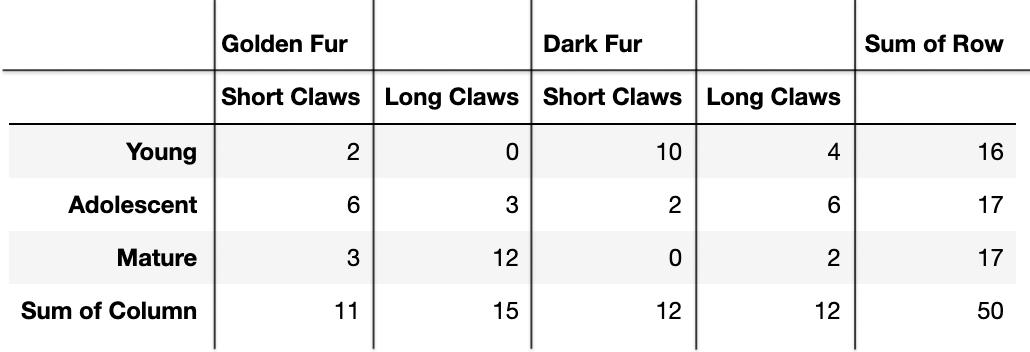
\includegraphics[width=0.9\textwidth]{final-images/su24_bayes.png}
    \end{center}

For instance, we're told that 10 cheetahs with dark fur and short claws are young and that there were 11 cheetahs with golden fur and short claws.

Given its other characteristics, San Diego Safari Park would like to use this information to predict whether a cheetah new to the Park is young, adolescent, or mature.

\bigskip


A new cheetah is observed with \textbf{golden fur} and \textbf{long claws}. Using the data in the table and assuming conditional independence of features, use the Naive Bayes formula \textbf{with smoothing} to determine which developmental stage is most likely for the new cheetah. In this question, you may leave your answers unsimplified, in terms of fractions, exponents, factorials, the permutation formula $P(n, k)$, and the binomial coefficient ${n \choose k}$.


 \begin{responsebox}{3.3in}
            
\end{responsebox}
    
    
\end{prob}

% LAST PAGE drawing
\newpage

Make sure you've written your PID in the space provided in the top right corner of every page of this exam. Congratulations on completing DSC 40A!

Feel free to draw us a picture about DSC 40A below. And here's a free point!

\begin{responsebox}{7.5in}
    
\end{responsebox}

\end{probset}

\end{document}
